6-1. 一平行板电容器的两极板都是半径为 $5.0\mathrm{cm}$ 的圆导体片，在充电时，其中电场强度的变化率为 $\frac{\mathrm{d}E}{\mathrm{d}t} = 1.0\times 10^{12}\mathrm{V / (m\cdot s)}$ 求：

(1) 两极板间的位移电流；

(2) 极板边缘的磁感应强度。

\vfill


6-2. 设电荷在半径为 $R$ 的圆形平行板电容器极板上均匀分布，且边缘效应可以忽略。把电容器接在角频率为 $\omega$ 的简谐交流电路中，电路中的传导电流为 $I_0$ （峰值），求电容器极板间磁场强度（峰值）的分布。

\vfill\newpage
6-3.如本题图，同心球形电容器中有介电常量为 $\varepsilon$ 和电导率为 $\sigma$ 的漏电介质。电容器充电后遂即缓慢放电，这时在介质中有径向衰减电流通过。求此过程中的位移电流密度与传导电流密度的关系，以及磁场的分布。

\begin{center}
    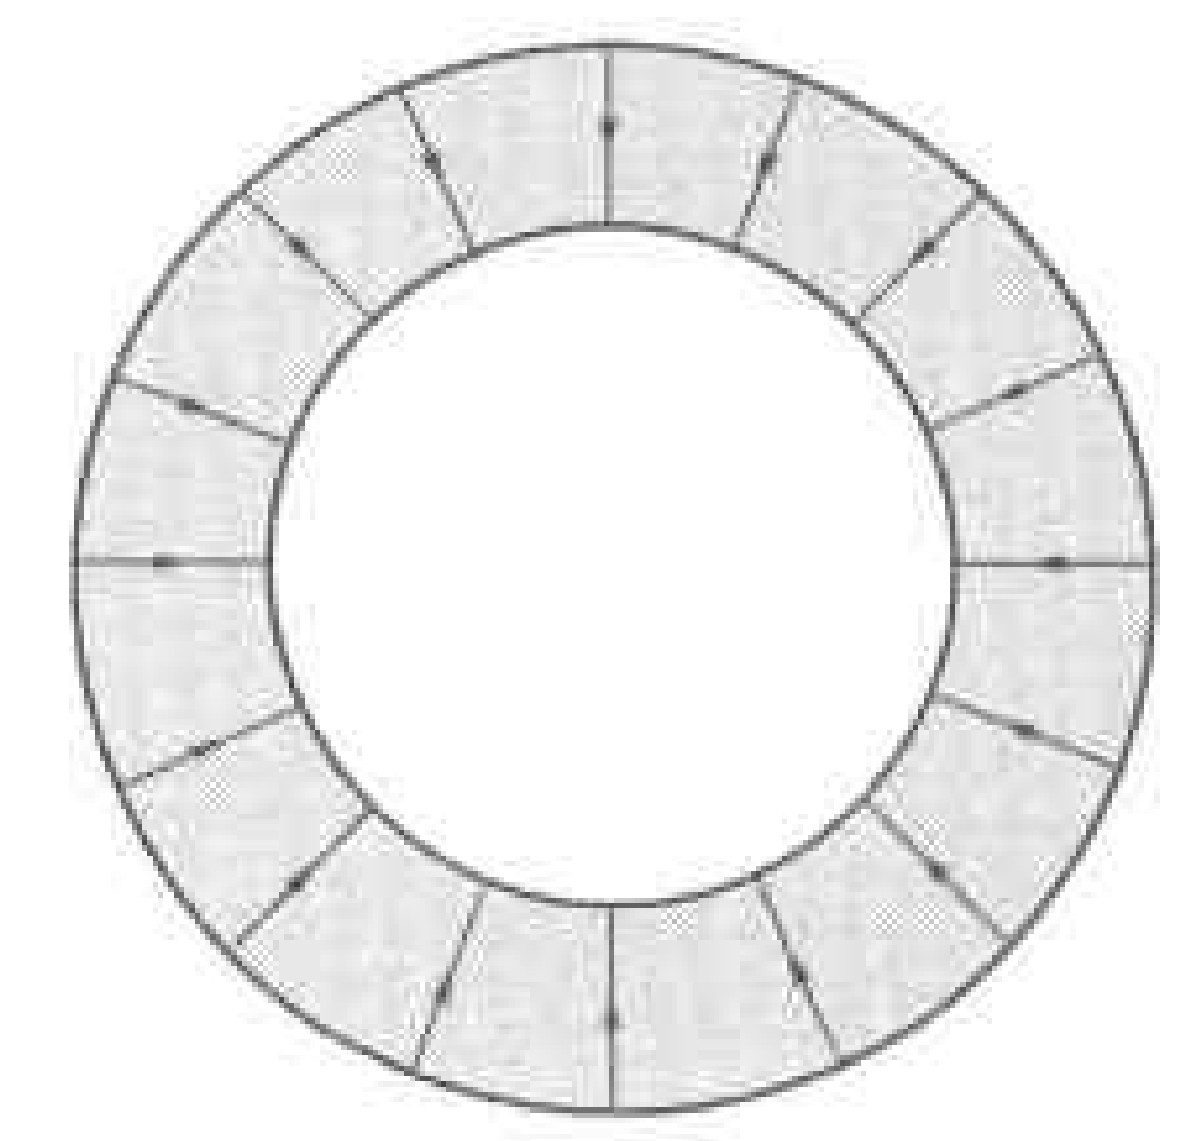
\includegraphics[width = 0.25\linewidth]{figures/习题6-3.jpg}
\end{center}
\vfill

6-4. 太阳每分钟垂直射于地球表面上每 $\mathrm{cm}^2$ 的能量约为 $2\mathrm{cal}(1\mathrm{cal}\approx 4.2\mathrm{J})$ ，求地面上日光中电场强度 $E$ 和磁场强度 $H$ 的方均根值。

\vfill\newpage
6-5.(1)作为典型的原子内部电场强度,试计算氢原子核在玻尔轨道处产生电场强度的数量级。(玻尔半径 $a_{B}=0.053nm$ .)

(2) 若要激光束中的电场强度达到此数量级, 其能流密度应为多少?

\vfill
6-6.本题图所示为太阳的结构模型，中心核约占 $0.25R_{\odot}$ ，是聚变反应区，密度为 $160\mathrm{g / cm^3}$ （太阳平均密度的114倍），温度为 $1.5\times 10^{7}\mathrm{K}$ .日核外面 $(0.25\sim 0.86)R_{\odot}$ 是辐射转移区，能量靠辐射和扩散向外传输。再外面是对流层、光球、色球和日冕。各层的辐射光压可用斯特藩-玻耳兹曼定律算出：
$$
p = \frac {1}{3} a T ^ {4},
$$

式中斯特藩-玻耳兹曼常量 $a=7.566\times10^{-16}\mathrm{J}/(\mathrm{m}^{3}\cdot\mathrm{K}^{4})$

(1) 估算太阳中心的光压和电磁辐射中电场强度；

（2）在辐射转移区内取半径为 $0.4R_{\odot}$ 处的温度为 $4.8\times10^{6}K$ ，求该处的光压和电磁辐射中电场强度；

(3) 将以上两问的电场强度与原子内部电场强度作数量上的比较。

\begin{center}
    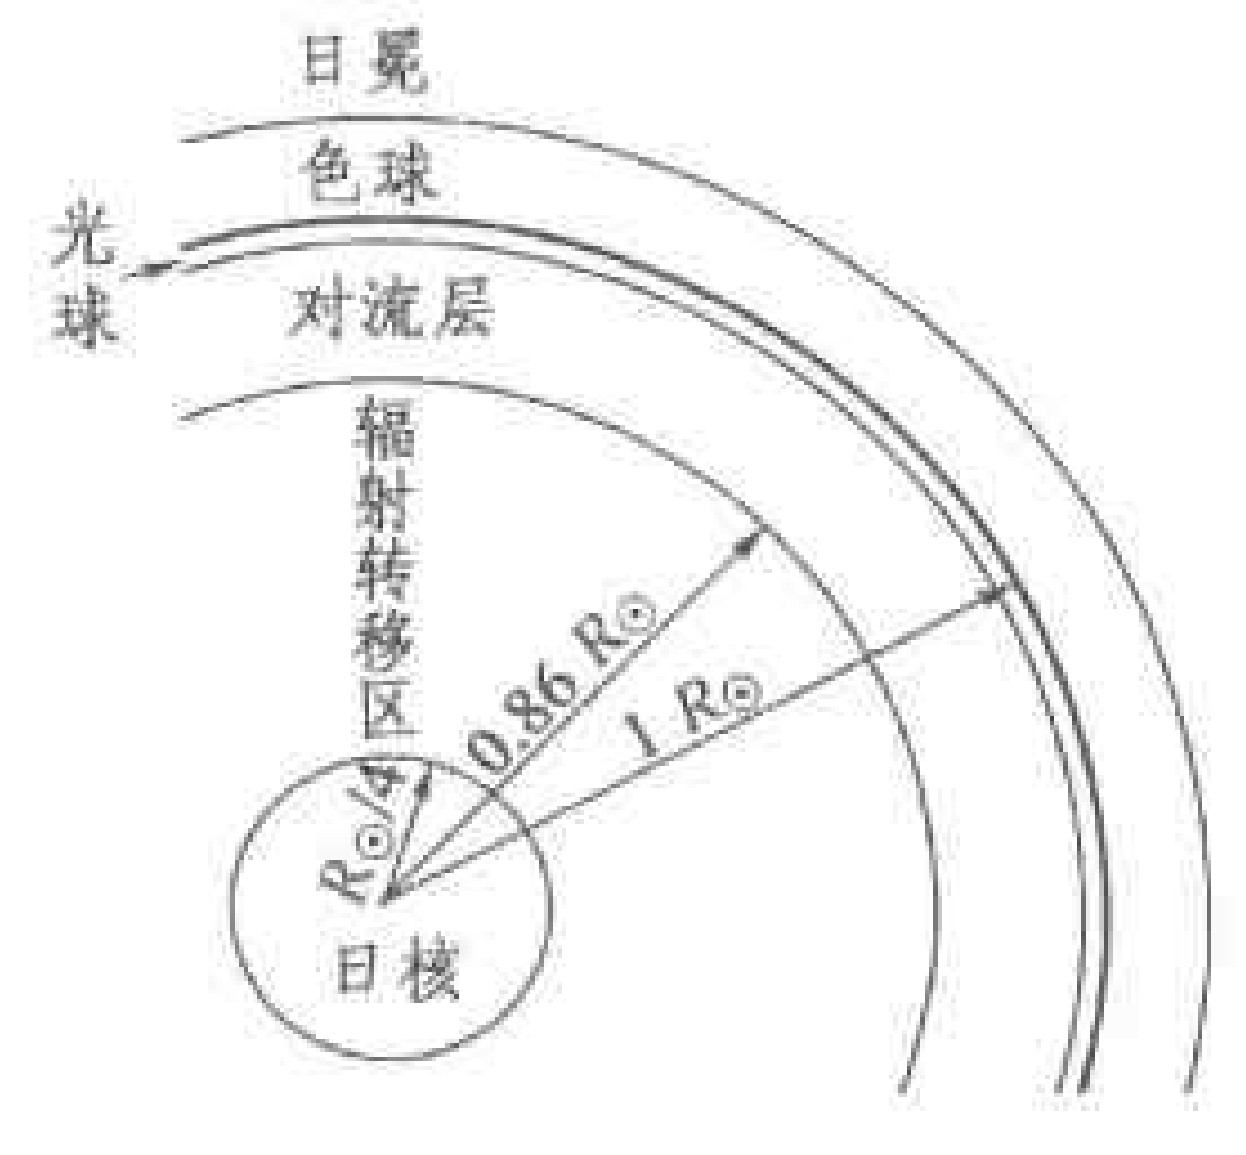
\includegraphics[width = 0.25\linewidth]{figures/习题6-6.jpg}
\end{center}
\vfill\newpage
6-7. 设 $100\mathrm{W}$ 的电灯泡将所有能量以电磁波的形式沿各方向均匀地辐射出去, 求:

(1)20m 以外的地方电场强度和磁场强度的方均根值；

(2) 在该处对理想反射面产生的光压。

\vfill
6-8. 设图 6-21b 或 c 中圆柱形导线长为 l，电阻为 R，载有电流 I. 求证:电磁场通过表面 $\Sigma$ 输入导线的功率 $\iint E \times H \cdot d\Sigma$ 等于焦耳热功率 $I^{2}R$ .
\begin{center}
    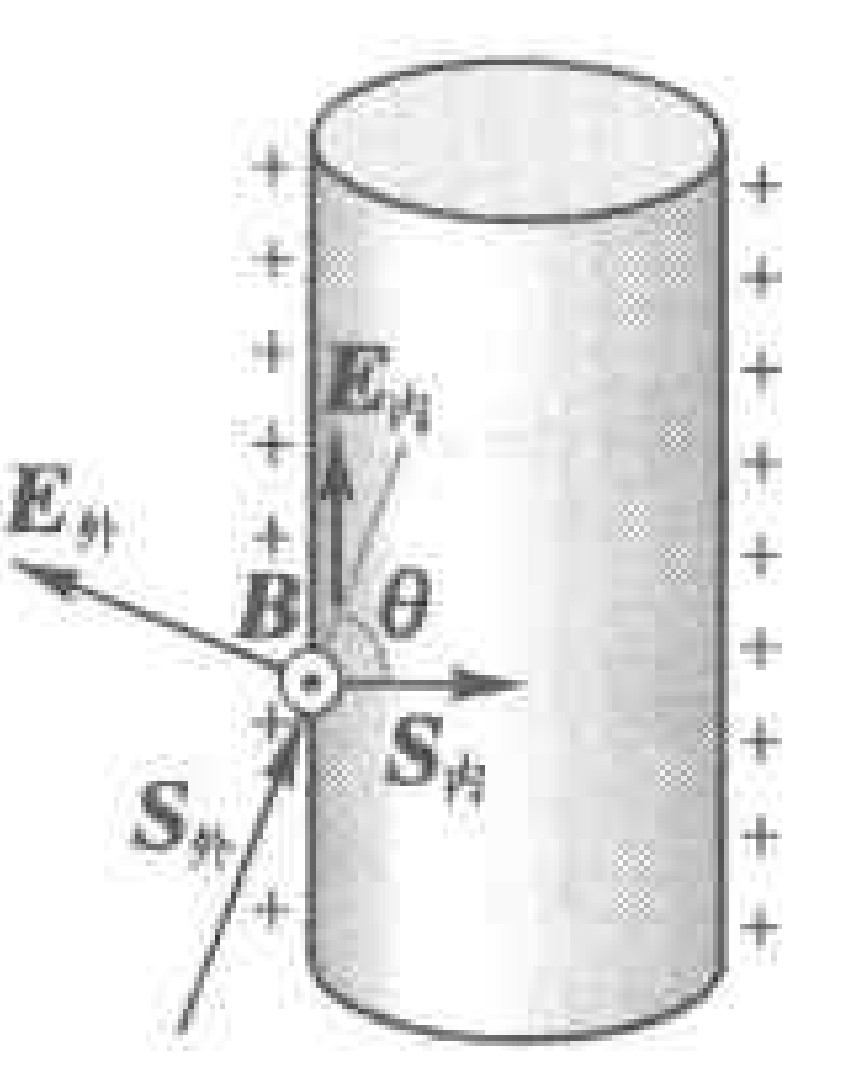
\includegraphics[width = 0.2\linewidth]{figures/习题6-8.jpg}
\end{center}
\vfill\newpage
6-9.本题图是一个正在充电的圆形平行板电容器，设边缘效应可以忽略，且电路是准恒的。求证：

(1) 坡印亭矢量 $S = E \times H$ 处处与两极板间圆柱形空间的侧面垂直；

(2) 电磁场输入的功率 $\iint E \times H \cdot d\Sigma$ 等于电容器内静电能的增加率，即 $\frac{d}{dt}\left(\frac{q^{2}}{2C}\right)$ ，式中 C 是电容量，q 是极板上的电荷量。
\begin{center}
    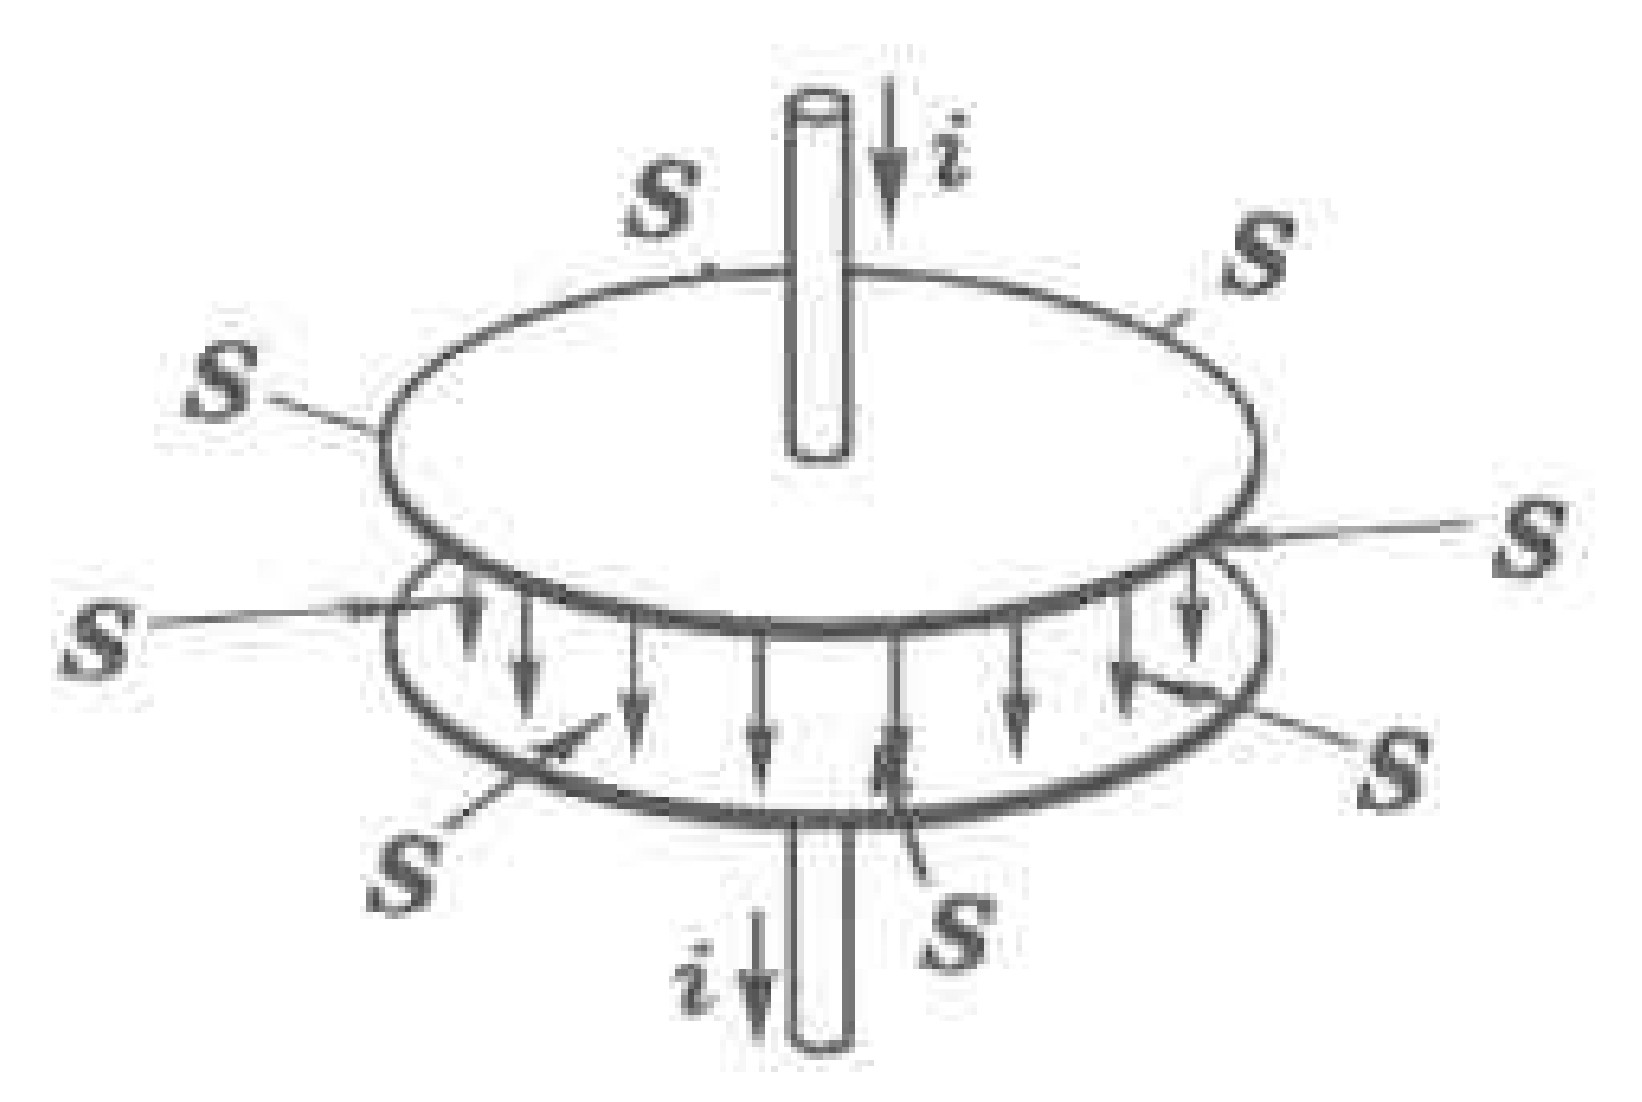
\includegraphics[width = 0.3\linewidth]{figures/习题6-9.jpg}
\end{center}
\vfill
6-10. 利用第一章习题1-59和第三章习题3-31的结果证明：在真空中沿平行双线传输线传播的电磁波速度为 $c$
\vfill\newpage
6-11. 利用电报方程证明: 长度为 $l$ 的平行双线(损耗可以忽略)两端开启时电压和电流分别形成如下形式的驻波:

$$
\left. \begin{array}{l} \widetilde {U} = \widetilde {U _ {0}} \cos \frac {p \pi x}{l} \exp (\mathrm{i} \omega_ {p} t), \\ \widetilde {I} = \widetilde {I} _ {0} \sin \frac {p \pi x}{l} \exp (\mathrm{i} \omega_ {p} t), \end{array} \right\} (p = 1, 2, 3, \dots)
$$
其中谐振角频率为 $\omega_{p}=\frac{p\pi}{l\sqrt{L^{*}C^{*}}}$ 。指出电压、电流的波腹和波节的位置，以及波长的大小。

【提示:假设电报方程的解是入射波和反射波的叠加,利用两端的边界条件确定驻波的谐振频率。】

\vfill
6 - 12. 上题中若传输双线两端短路, 情况若何?
\vfill
6 - 13. 上题中若传输双线一端开启、一端短路，情况若何？
\vfill\newpage
6-14. 推导高斯单位制中电能密度 $w_{\mathrm{e}}$ 、磁能密度 $w_{\mathrm{m}}$ 、坡印亭矢量 $S$ 和电磁动量密度 $g$ 的表达式。
\vfill
6-15. 推导高斯单位制中平行板电容器电容和螺线管自感的表达式。
\vfill\newpage
6-16. 实用中磁场强度的单位往往用 Oe, 而电流的单位用 A, 长度的单位用 cm (这是 MKSA 制和高斯制的混合)。试证明, 在这种情况下螺线管磁场强度的公式为 $H = 0.4\pi nI$
\vfill

6-17. 实用中磁通量的单位常常用 $\mathrm{Mx}$ , 电动势的单位用 V. 试证明: 在这种情况下法拉第电磁感应定律的表达式为
$$
\mathcal {E} = - 1 0 ^ {- 8} \frac {\mathrm{d} \Phi_ {B}}{\mathrm{d} t}.
$$
\vfill\newpage